\section{Appendix}
\subsection{Pictures to the Personas}

\begin{figure}[H]
  \centering
  \subfloat[Jeff and Judy Seavers]{\label{fig:seavers}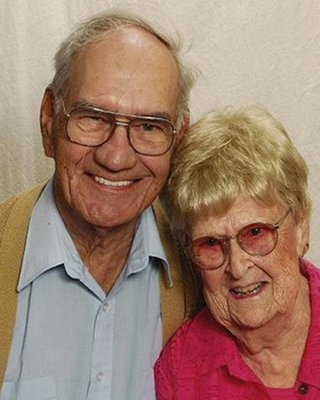
\includegraphics[width=0.3\textwidth]{Images/jeff_and_judy_seavers.jpg}}                
  \subfloat[Sarah Gordon]{\label{fig:gordon}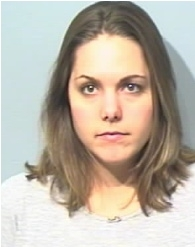
\includegraphics[width=0.3\textwidth]{Images/sarah_gordon.jpg}}
  \subfloat[Bruce Walker]{\label{fig:walker}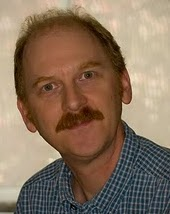
\includegraphics[width=0.3\textwidth]{Images/bruce_walker.jpg}}
  \caption{Personas}
  \label{fig:personas}
\end{figure}

\subsection{User Involvement Methods}
\subsubsection{Accompanying letter}\label{sec:letter}
Dear \dots

For our course "Human Computer Interaction", we have to design a system for selling baby clothes. Our group decided to build a web-based system, for which we need your help. In order to find out about which features our system should include, we made a questionnaire with some questions concerning web shops (in general and clothes/baby clothes in particular).
If you can spare fifteen minutes of your time, we'd greatly appreciate if you could help us and fill out the questions.

Thank you very much!\\
Alban Edouard, Gianin Basler, Irem Tanriseven, Joana Welti


\newpage
\subsubsection{Questionnaires}

\minisec{Draft}
\begin{figure}[H]
\begin{center}
\includegraphics[scale=0.75]{User_Involvement_Methods/Questionnaires/Questionnaire_Web_Shops_v2_1.png}
\end{center}
\end{figure}
\newpage
\begin{figure}[H]
\begin{center}
\includegraphics[scale=0.75]{User_Involvement_Methods/Questionnaires/Questionnaire_Web_Shops_v2_2.png}
\caption{Questionnaire First Draft}
\label{fig:draft}
\end{center}
\end{figure}

\minisec{Explanations}\label{sec:explanations}
The \textit{personal information} questions aim at finding out more about the person filling out the questionnaire. With these questions, we want to find with what kind of person (parent, age, experience etc.) we are dealing with. The \textit{web shops in general} section tries to find out more about the person's online shopping behavior. Especially, we would like to know if people mind to create an account when ordering items online, if wishlists are a feature that is actually used and what other features are valued most by users.
We also ask some more specific questions concerning clothes web shops to find out what the problems are when buying clothes online so that we can enhance our shop with features to make it easier to buy clothes online. 
Last, we have a few questions about \textit{baby clothes shops} in particular. We would like to include the feature that people can buy and sell used clothes online and we would like to know if users consider this useful. Also, we aren't sure how much help people need when deciding on the right size for baby clothes, so we have another question concerning selecting the correct size. 

\minisec{Improvements}\label{sec:improvements}
 In the introduction part, we added a simple question for the example in addition to the response. For the questions 3 and 12.a, instead of repeating the previous question, we just wrote "if yes", which is clearer. The fourth question was entirely rewritten because some people didn't understand the "computing expertise" term. In questions 6 and 10, "store" was replaced "shop" to keep the terminology consistent. The last update was the recasting of the question 11 and the inversion of its scale of values, from 1 = "not useful" to 5 = "very useful", because this seems to be more natural to people. 

\begin{figure}[H]
\begin{center}
\includegraphics[scale=0.75]{User_Involvement_Methods/Questionnaires/Questionnaire_Web_Shops_v3.pdf}
\end{center}
\end{figure}
\newpage
\begin{figure}[H]
\begin{center}
\includegraphics[scale=0.75]{User_Involvement_Methods/Questionnaires/Questionnaire_Web_Shops_v3_2.pdf}
\caption{Questionnaire Final Version}
\label{fig:final}
\end{center}
\end{figure}
\newpage

\subsubsection{Contextual Inquiry}\label{sec:contextual_inquiry}
Website used: \url{http://www.oshkoshbgosh.com/}

\paragraph{Questions before the task}
\begin{itemize}\addtolength{\itemsep}{-0.5\baselineskip}
 \item Did you ever buy clothes for children?
 \item Have you ever bought clothes online?
 \item What webshop do you use?
 \item What do you like about these shops?
 \item Do you have accounts for the shops you use regularly?
 \item What payment method do you prefer?
\end{itemize}


\paragraph{Tasks}
\begin{itemize}\addtolength{\itemsep}{-0.5\baselineskip}
 \item \textbf{Boy}
 \item Aged 2 years
 \item Yellow shirt, as cheap as possible
\end{itemize}
\begin{itemize}\addtolength{\itemsep}{-0.5\baselineskip}
 \item Girl
 \item Aged 2 months
 \item White dress, but with some flowers on it
 \item Price not important
\end{itemize}
\begin{itemize}
 \item Change quantity from 1 to 2 for the dress
\end{itemize}

Look for:
\begin{itemize}\addtolength{\itemsep}{-0.5\baselineskip}
 \item Is ``filter by'' used?
 \item Way to get to product?
 \item Search bar used? What were the search terms?
\end{itemize}

\paragraph{Questions for interview after task}
\begin{itemize}\addtolength{\itemsep}{-0.5\baselineskip}
 \item Hidden or easy to find?
 \item How did you decide on a size for the dress?
 \item How do you like the web site?
 \item What would you improve on the site?
\end{itemize}

\newpage

\minisec{Explanations}\label{sec:inquiry_explanations}
The \textit{first questions} are designed to find out some background information about our inquired person in terms of their previous experiences with web shops. 

Our \textit{task descriptions} ask the inquired person to perform three different tasks. The first one has its focus on finding an item as cheap as possible, where the second one asks for a very specific item. 

While our inquired person does our tasks, we want to see how they find the products in order to learn more about how people navigate on a web shop. We also want to look for if the ``filter by'' and the search functionality is used to find out how we can include them in the most useful way in our project. 
 
The \textit{questions afterwards} focus on the experience the inquired person had.

\subsubsection{Proofs}
All the filled in questionnaires and the inquiry protocols can be found on github:
\url{https://github.com/joanawelti/Human-Computer-Interaction-Project-AGIJ/tree/master/User_Involvement_Methods/Questionnaires/Replays}

\minisec{Proof Picture}
\begin{figure}[H]
\centering
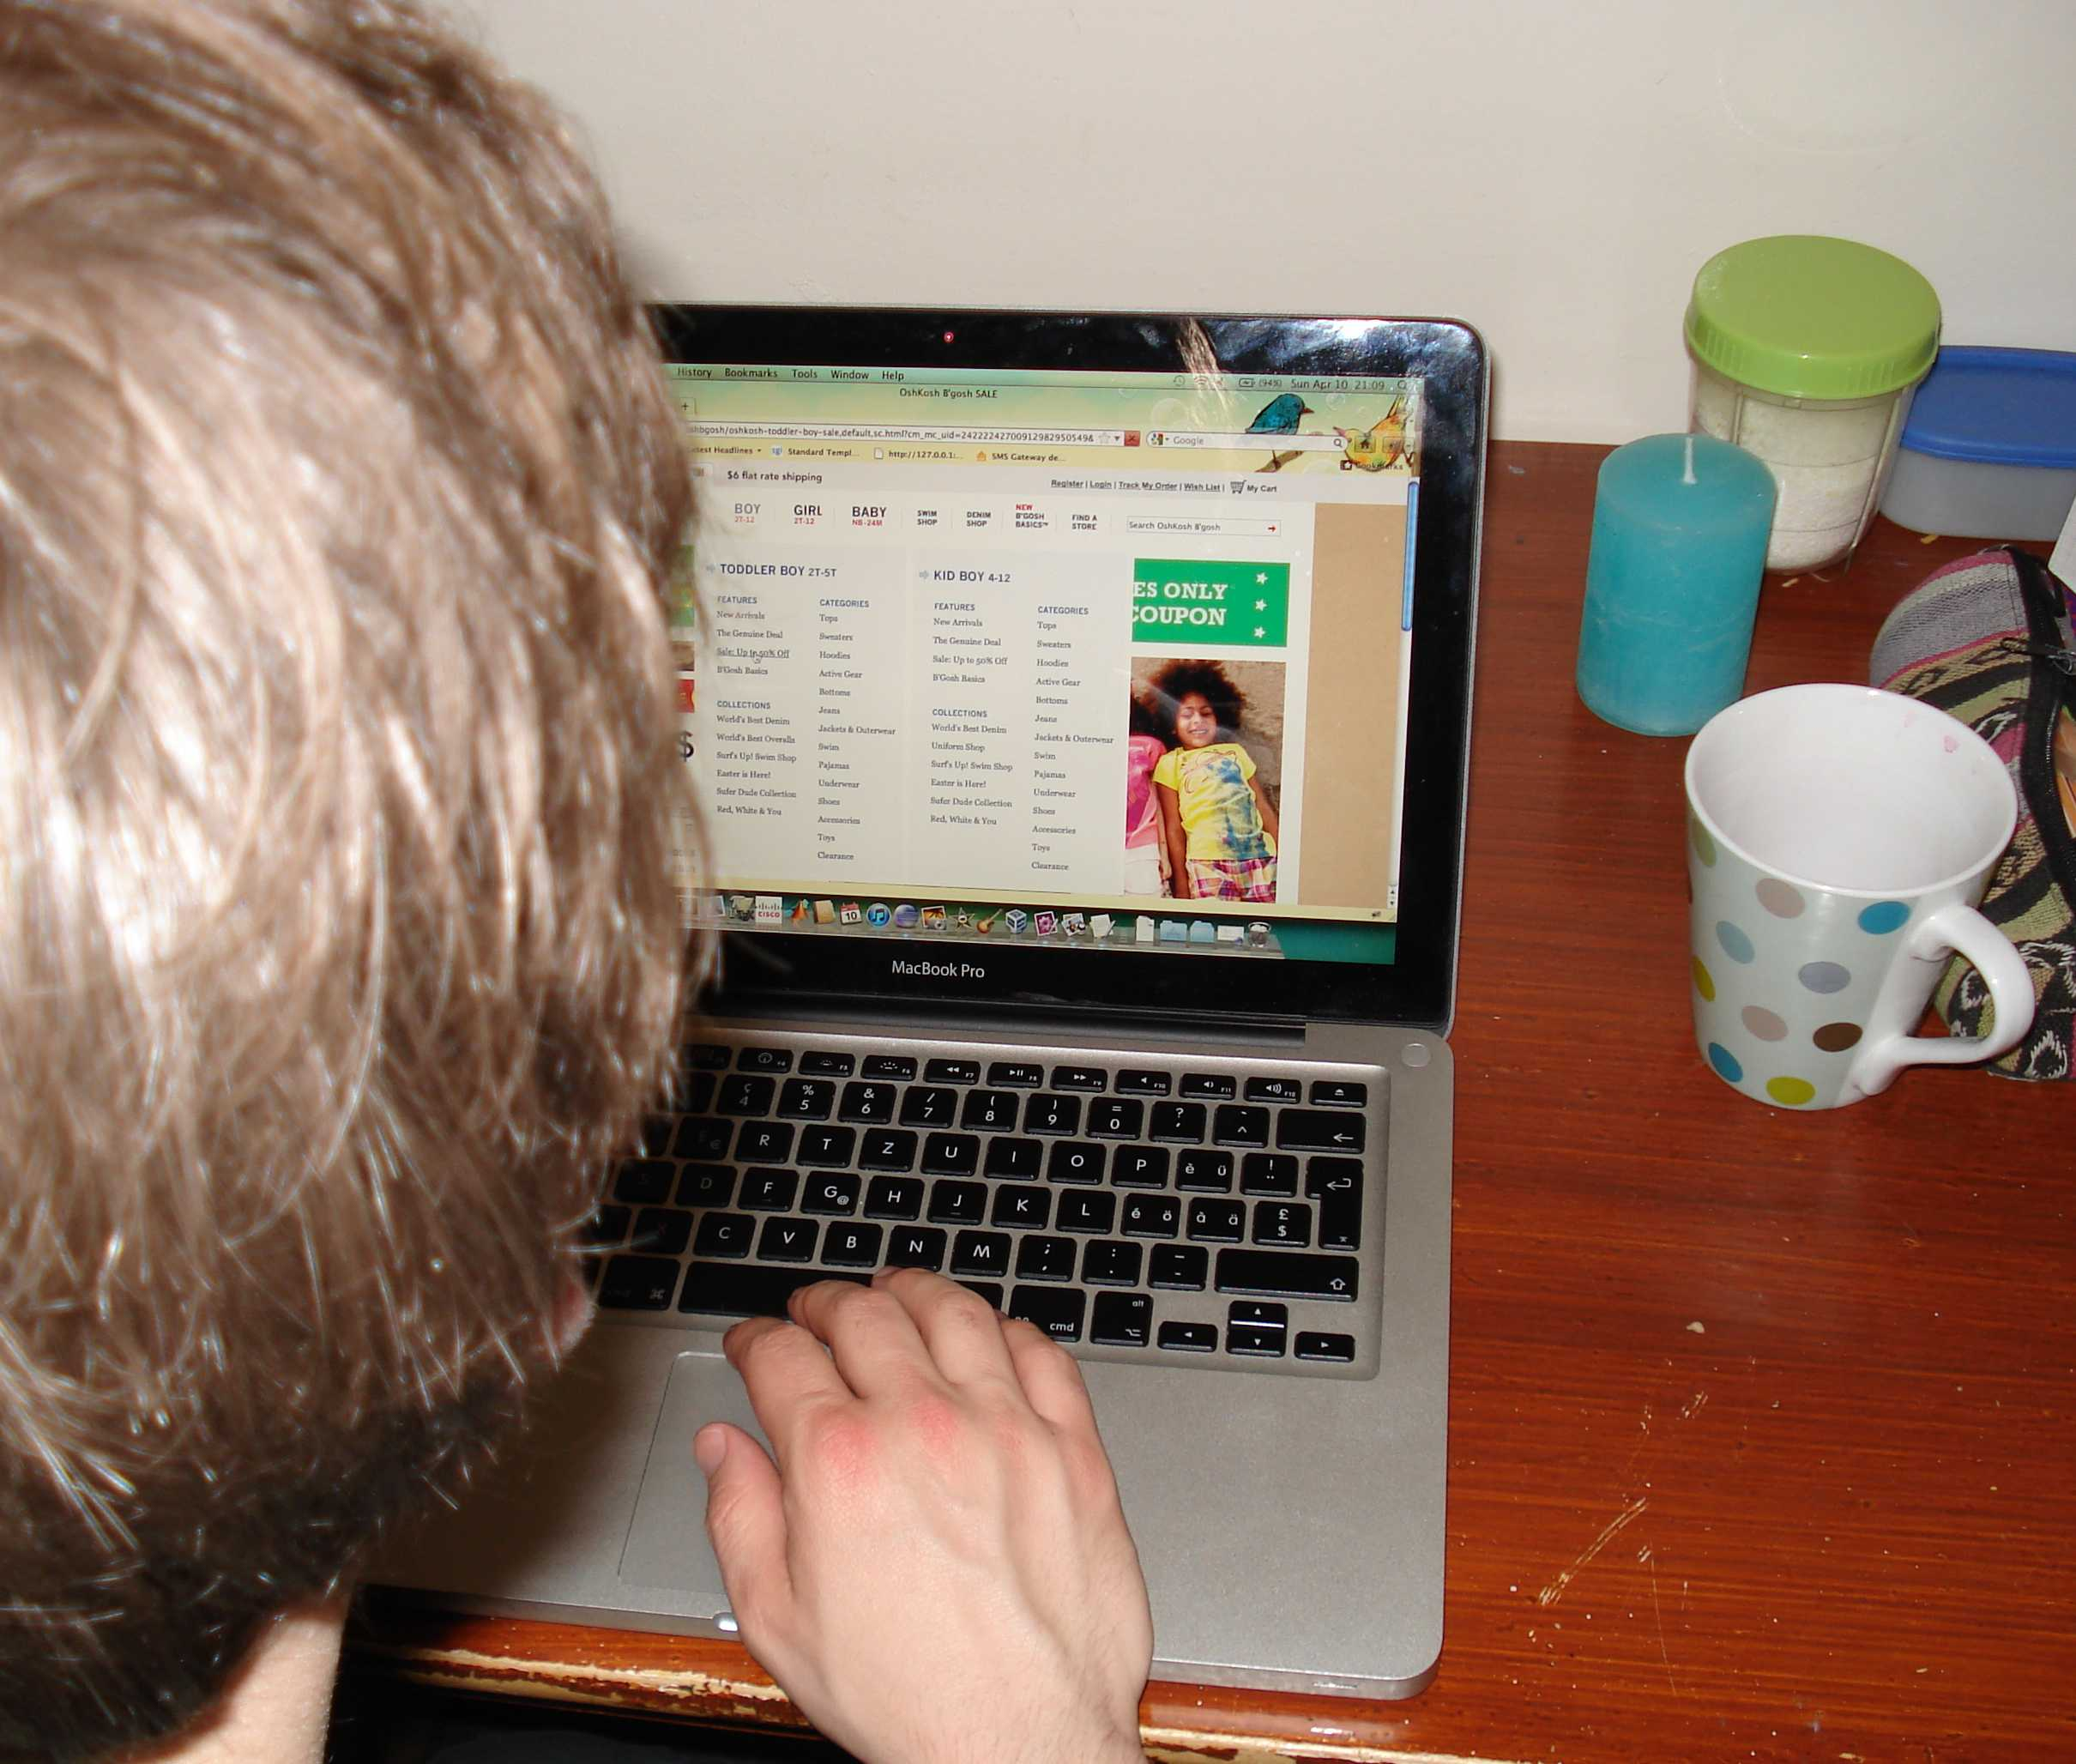
\includegraphics[width=8cm]{Images/inquiry_bjoern.JPG}
\caption{Inquiry with Bj\"orn}
\label{fig:inquiry_bjoern}
\end{figure}


\subsection{Navigation}
\begin{figure}[H]
  \centering  
  
\includegraphics[width=0.5\textwidth]{Images/globalMenu.jpg}                
  \caption{Global navigation menu}
  \label{fig:globalMenu}
\end{figure}

\begin{figure}[H]
  \centering
  \subfloat[Sublocal menu for Tops]{\label{fig:localMenuTops}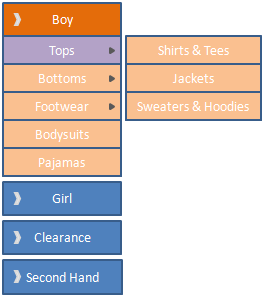
\includegraphics[width=0.35\textwidth]{Images/localMenuTops.png}}                
  \subfloat[Sublocal menu for Bottoms]
  {\label{fig:localMenuBottoms}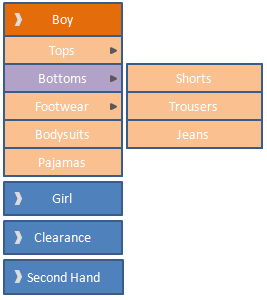
\includegraphics[width=0.35\textwidth]{Images/localMenuBottoms.png}}
  \subfloat[Sublocal menu for Footwear]{\label{fig:localMenuFootwear}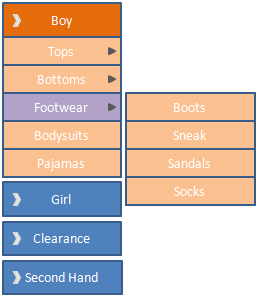
\includegraphics[width=0.35\textwidth]{Images/localMenuFootwear.png}}
  \caption{Local menu for Boys}
  \label{fig:localMenu}
\end{figure}

\newpage

\subsection{Prototype}
Note that the user review handling is not included in the screen shots, as this is not important for the core functionality.

\begin{figure}[H]
\begin{center}
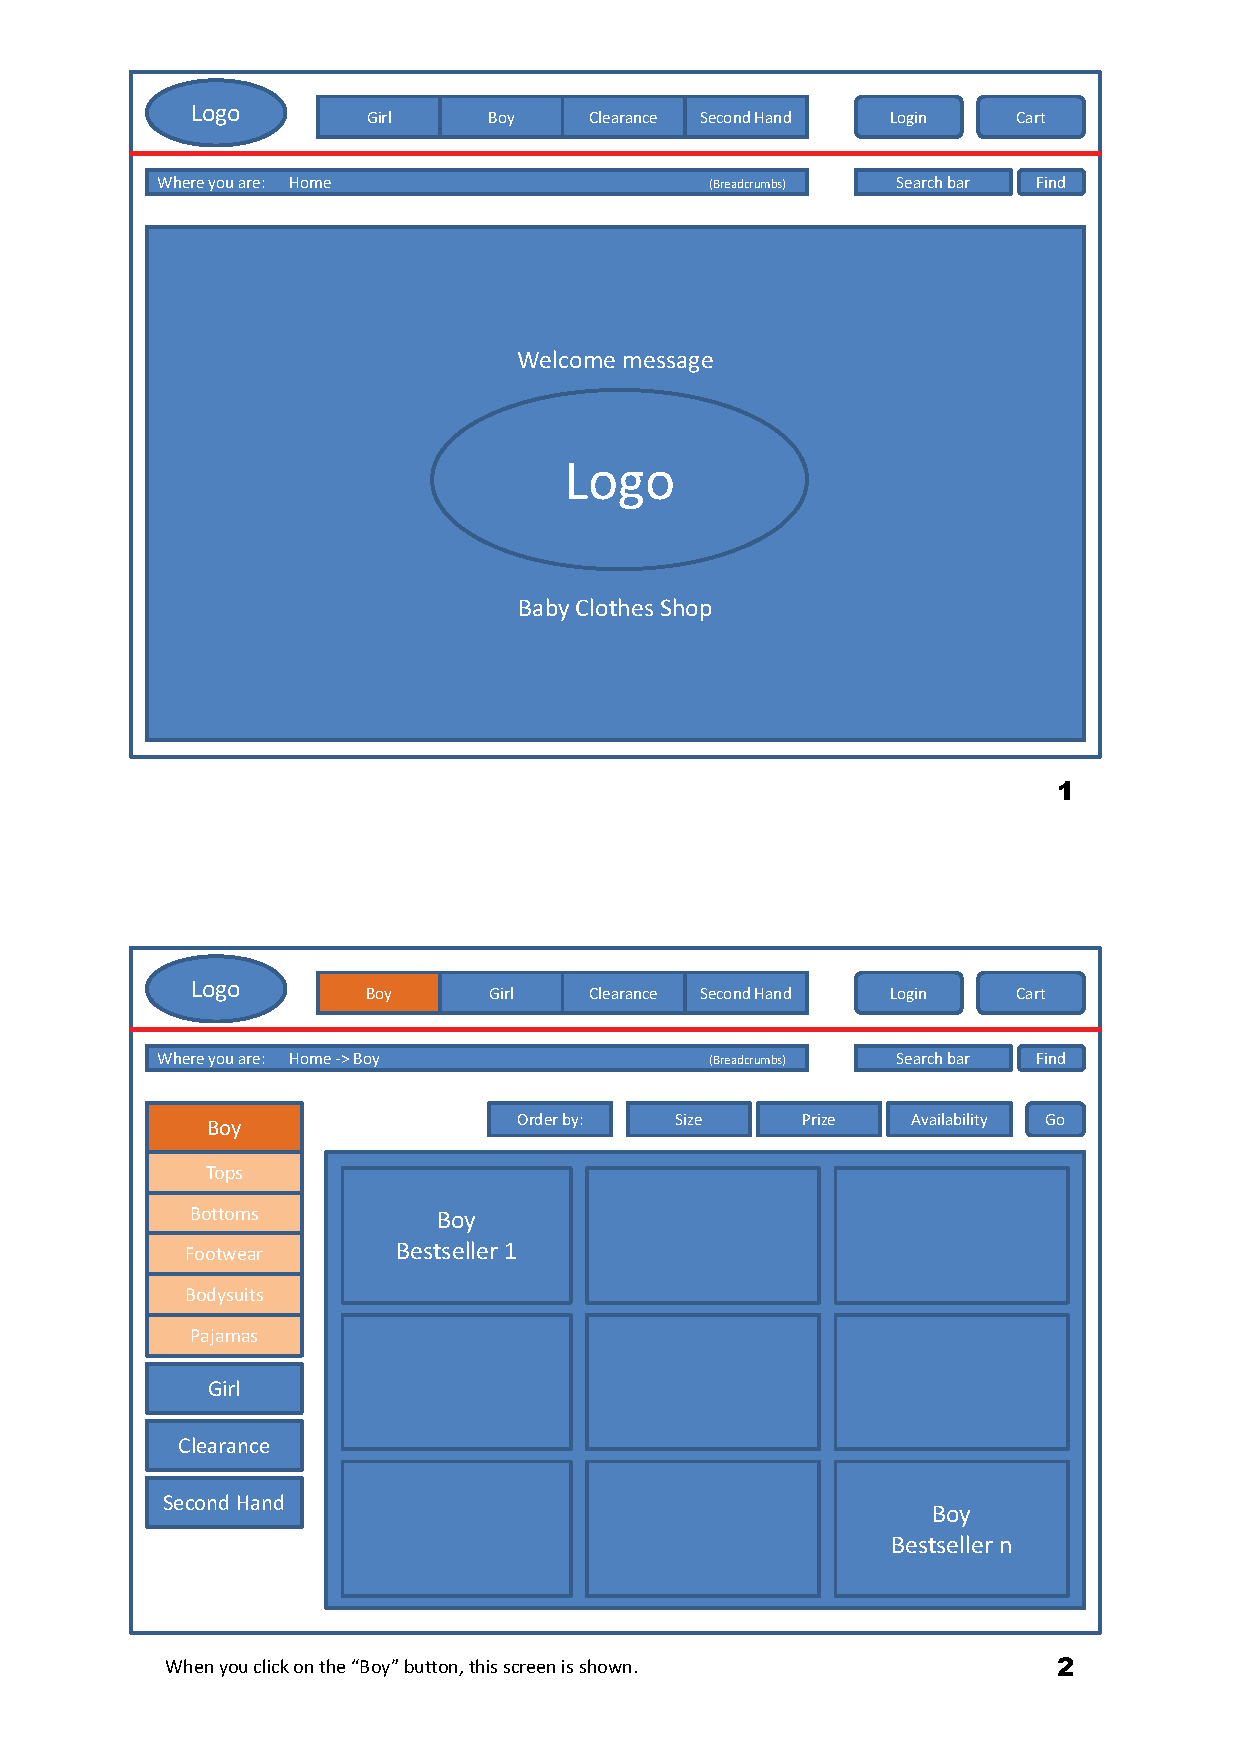
\includegraphics[scale=0.77]{Prototype/HCI_Prototype_2_1_1.png}
\end{center}
\end{figure}
\newpage
\includepdf[pages=2-8]{Prototype/HCI_Prototype_2_1.pdf}

\newpage

\subsection{Analytical Usability Evaluation Results}
\begin{figure}[H]
\begin{center}
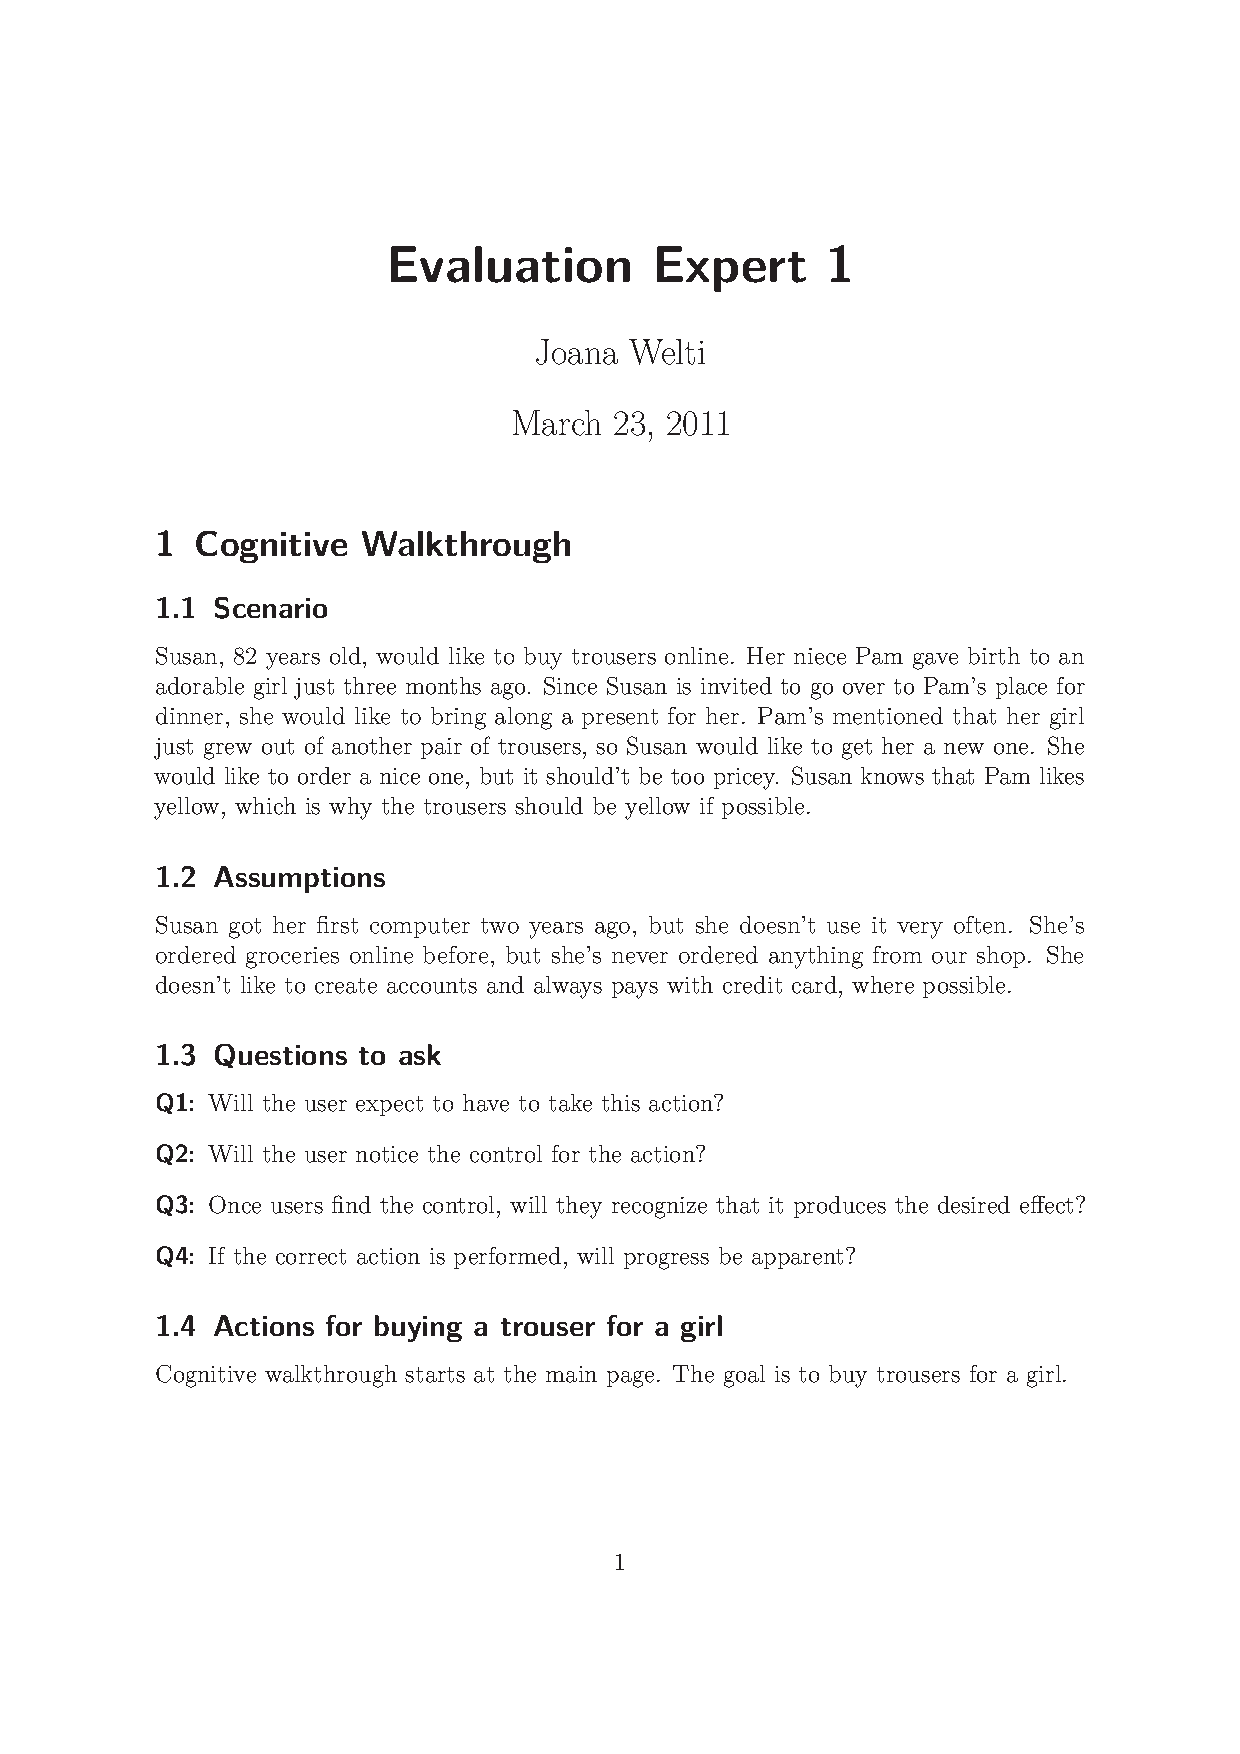
\includegraphics[scale=0.77]{Analytical_Usability_Evaluation/cognitive_walkthrough_joana_1.png}
\end{center}
\end{figure}
\newpage
\includepdf[pages=2-5]{Analytical_Usability_Evaluation/cognitive_walkthrough_joana.pdf}
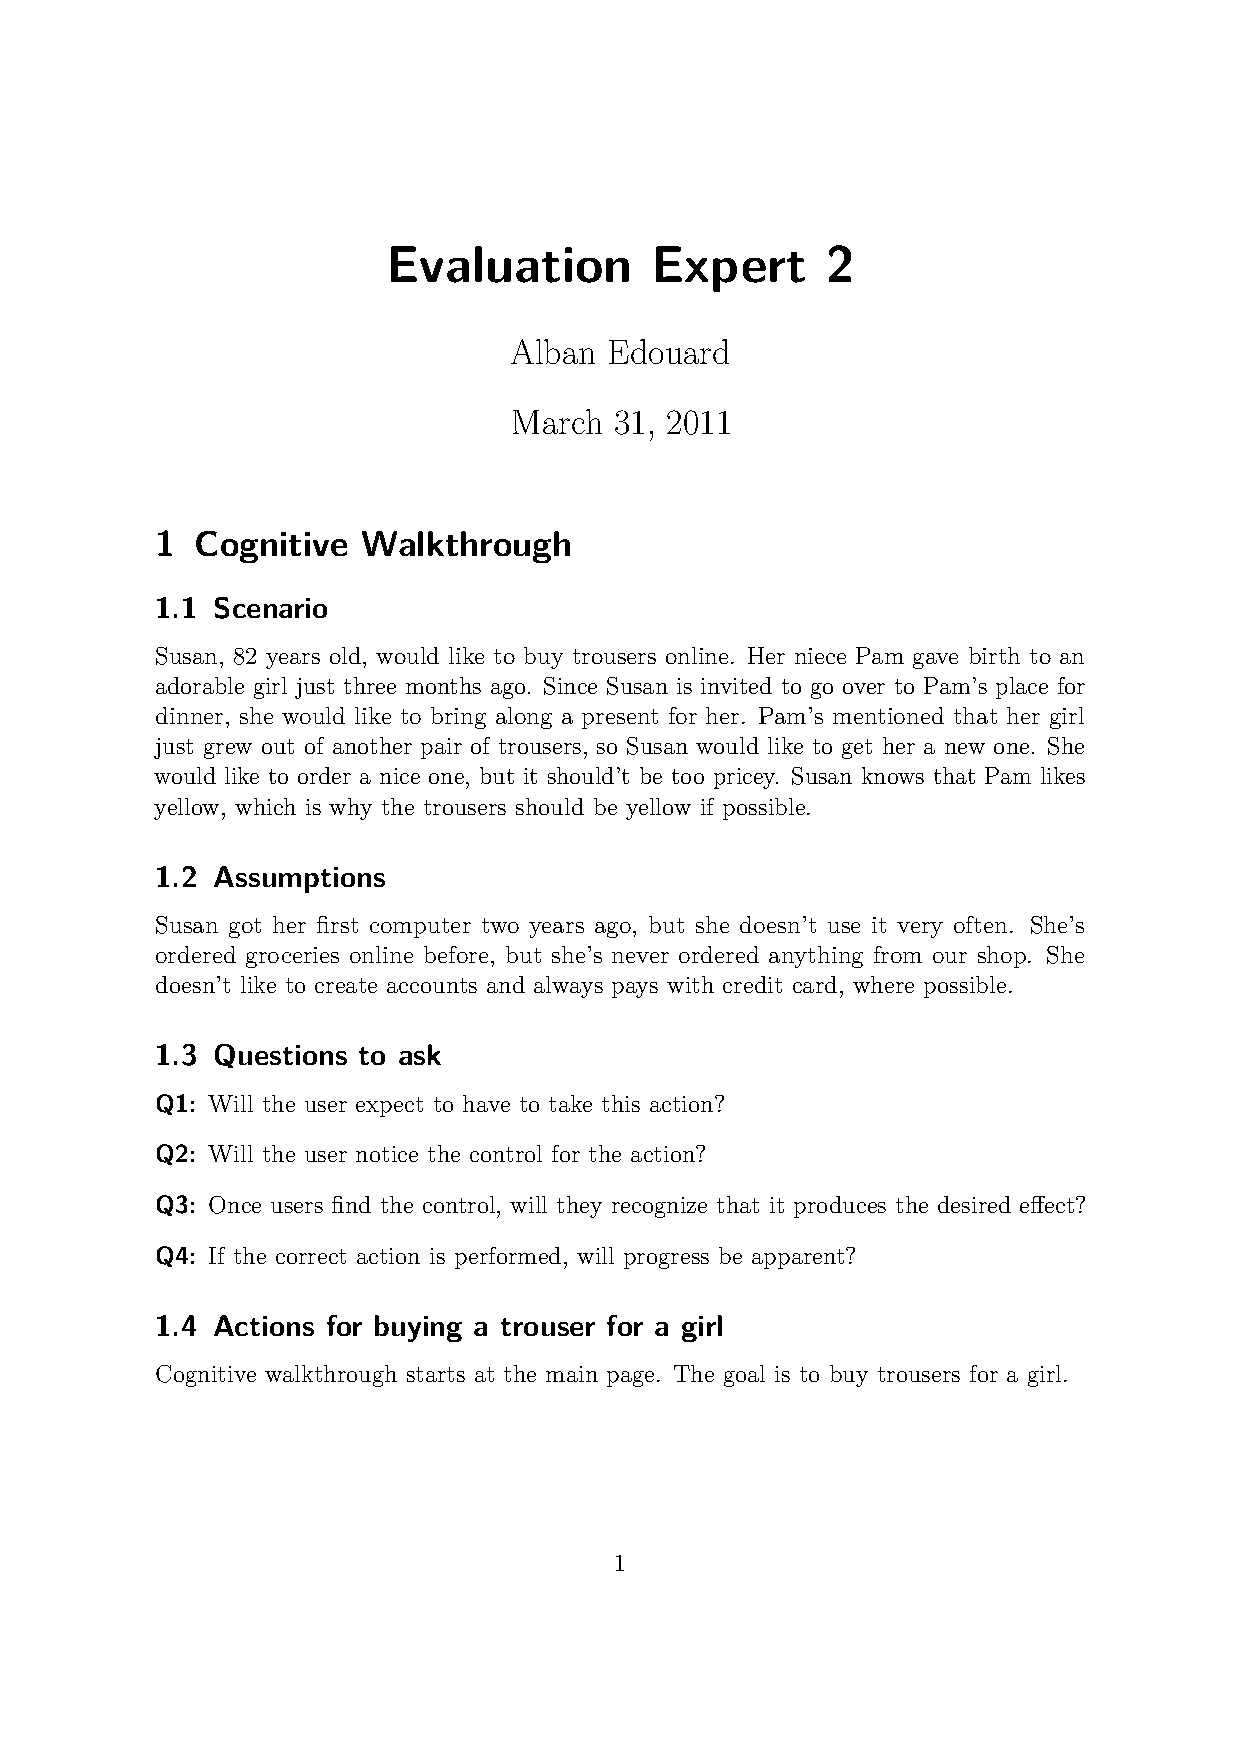
\includepdf[pages=-]{Analytical_Usability_Evaluation/cognitive_walkthrough_alban.pdf}
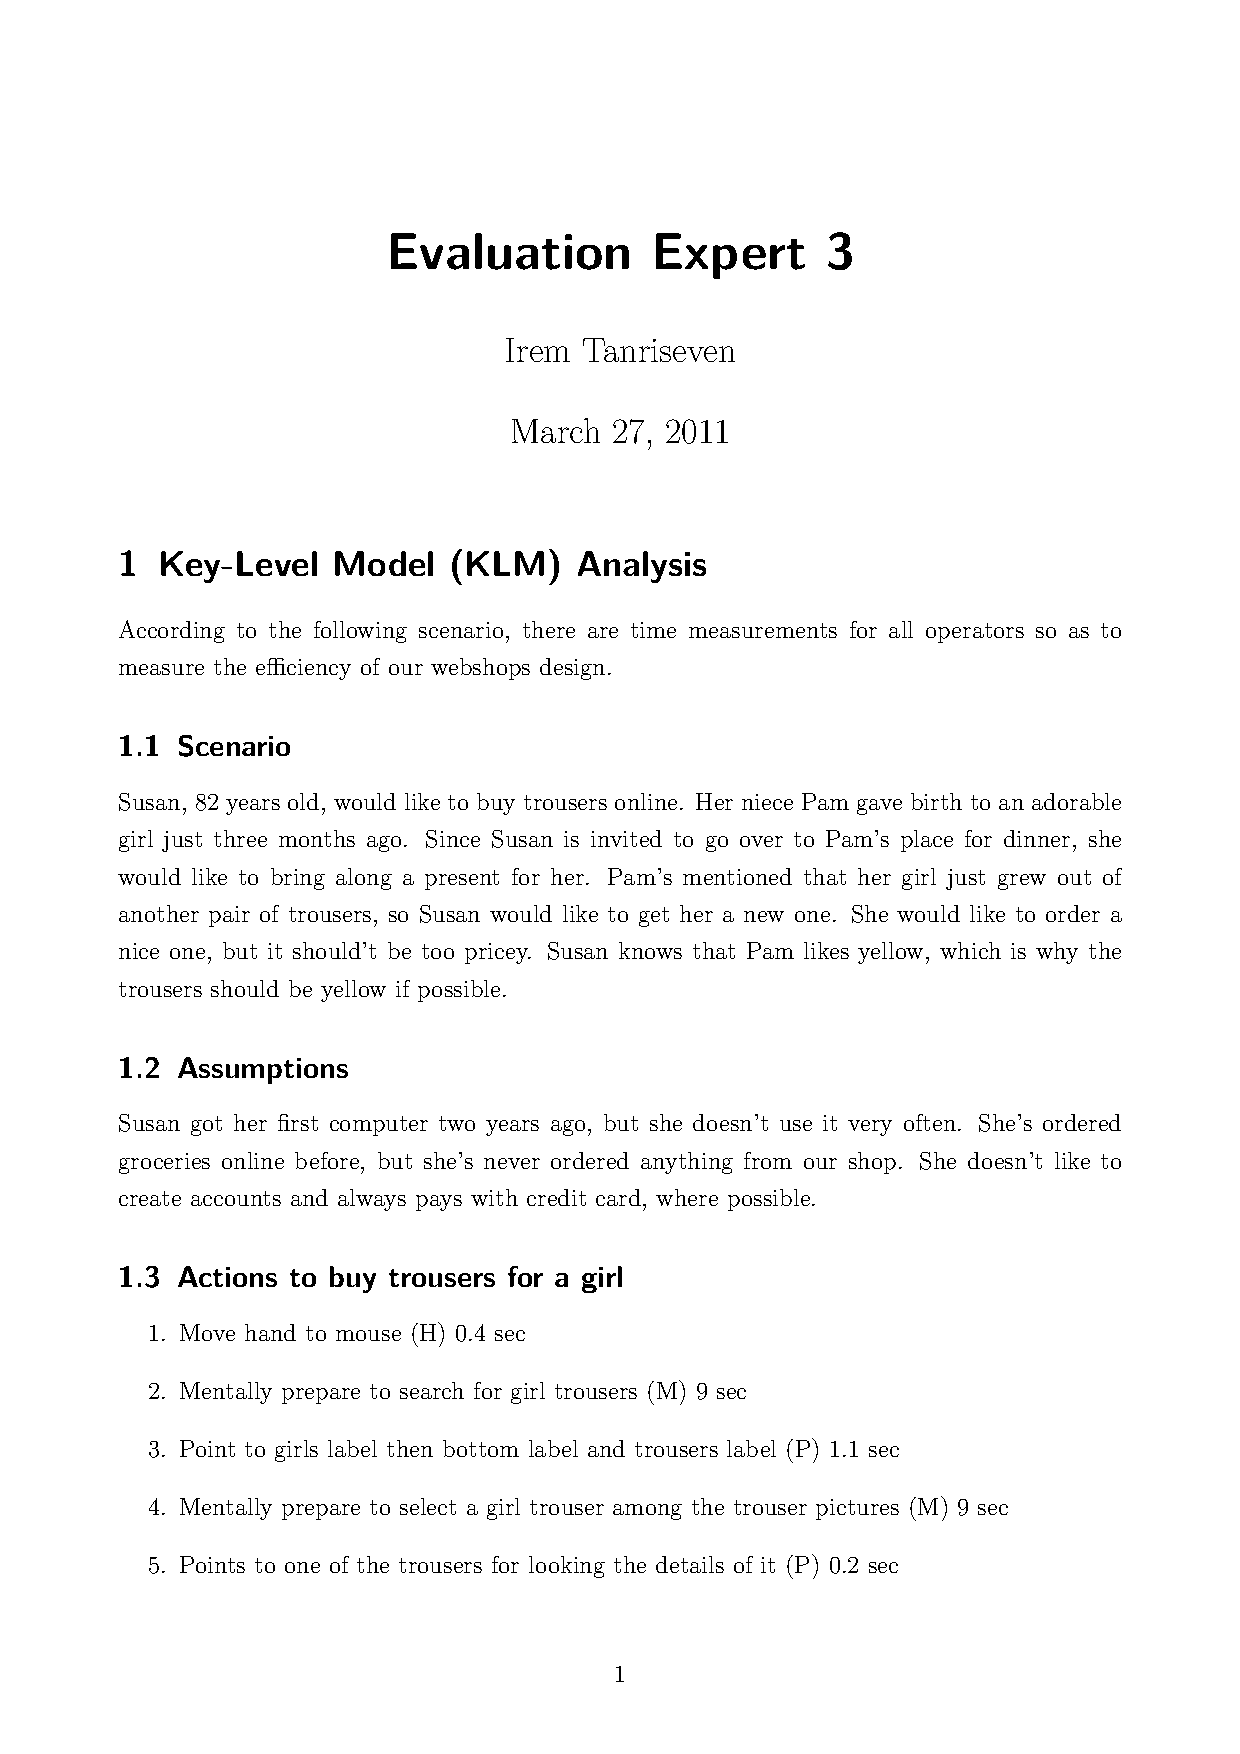
\includepdf[pages=-]{Analytical_Usability_Evaluation/KLM_Analysis_irem.pdf}